
\chapter
{The PEBL Launcher}

The PEBL Launcher is the recommended way to run PEBL experiments,
manage studies, and configure experiment chains.  It provides a
graphical interface for researchers and research assistants to launch
individual tests, build multi-test sequences, edit parameters, and
review output logs.

\begin{figure}[h]
\caption{The PEBL Launcher --- Manage Studies view.}
\center
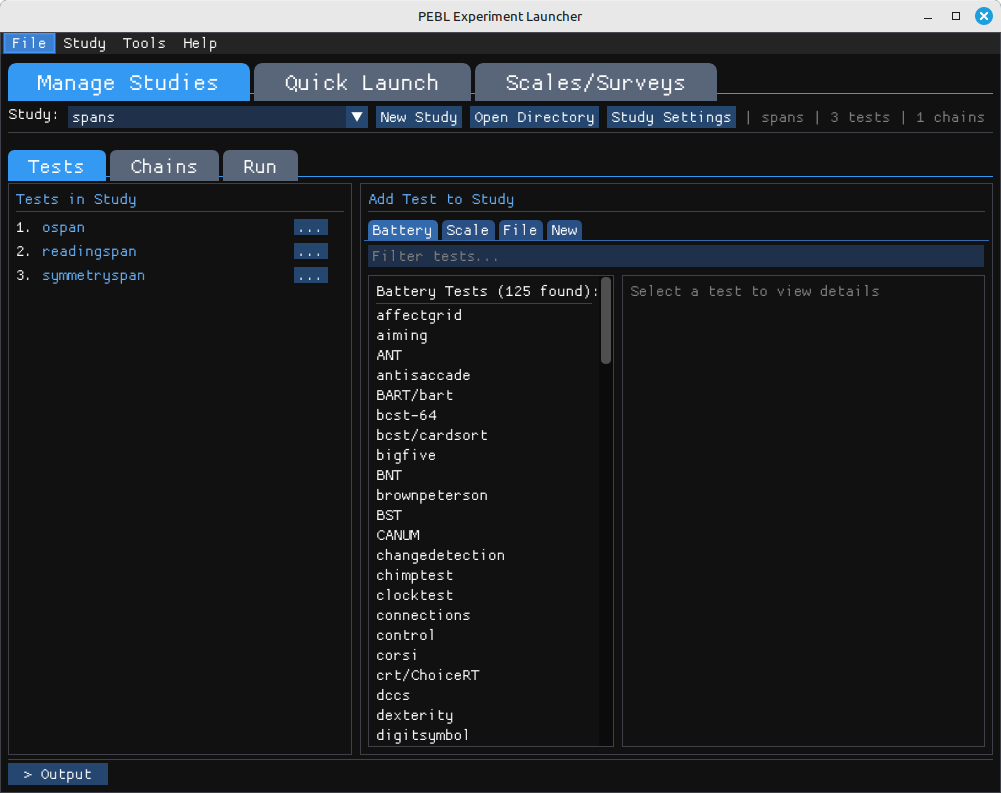
\includegraphics[width=0.9\textwidth]{images/launcher-overview.png}
\end{figure}
\clearpage


\sect{History of the Launcher}

Prior to PEBL 0.12, a front-end launcher was only available on Windows,
written in Visual Basic 6.  Starting with version 0.12, the launcher
was rewritten in PEBL itself, which made it cross-platform and
dependency-free.  Version 0.14 added custom GUI objects (buttons,
scrollboxes, menus, etc.) for a more polished interface.

For PEBL 2.4, the launcher was completely rewritten in C++ using the
\href{https://github.com/ocornut/imgui}{Dear ImGui} immediate-mode GUI
library and SDL2.  This native launcher replaces the earlier
PEBL-script-based launcher.  It is significantly faster to start, more
responsive, and supports features (study management, snapshot sharing,
built-in scale/survey editor) that were not practical in the
script-based approach.  The native launcher is distributed as part of
the standard PEBL AppImage package on Linux, and as \texttt{pebl-launcher.exe}
in the Windows installer.


\sect{Starting the Launcher}

\subsection{Linux (AppImage)}

When you run the AppImage directly (double-click or without a symlink
name), the GUI launcher starts automatically:
\begin{verbatim}
./PEBL-2.4-x86_64.AppImage
\end{verbatim}
If you have installed the system-wide symlinks described in the
Installation section, you can also run:
\begin{verbatim}
pebl-launcher
\end{verbatim}

\subsection{Windows}

Run \texttt{pebl-launcher.exe} from the \texttt{bin\textbackslash}
directory of your PEBL installation, or use the Start Menu shortcut
created by the installer.

\subsection{Installed vs.\ Portable Mode}

The launcher supports two operating modes:

\begin{description}
\item[Installed mode (default)] The workspace is created at
  \texttt{\textasciitilde/Documents/pebl-exp.2.4/} (Linux/Mac) or
  \texttt{My Documents\textbackslash pebl-exp.2.4\textbackslash} (Windows).
  On first run, the launcher offers to copy documentation, demos, and
  tutorials into this workspace.

\item[Portable/standalone mode] The workspace is the current working
  directory.  Portable mode is triggered by the presence of a
  \texttt{STANDALONE.txt} marker file in or near the executable directory,
  by a \texttt{PORTABLE.txt} file (legacy), or by setting the environment
  variable \texttt{PEBL\_PORTABLE=1}.  This mode is intended for
  USB-drive distributions or pre-configured research deployments.
  A typical portable layout looks like:
\begin{verbatim}
  MyPEBLDistribution/
    STANDALONE.txt       <- triggers portable mode
    runme.bat            <- Windows launch script (sets CWD first)
    PEBL/
      bin/pebl-launcher.exe
      bin/pebl2.exe
      battery/
      pebl-lib/
      media/
    my_studies/
    snapshots/
\end{verbatim}
\end{description}


\sect{Interface Overview}

The launcher window is divided into top-level tabs:

\begin{description}
\item[Manage Studies] The primary workspace for researchers.  Contains
  sub-tabs for Tests, Chains, and Run.
\item[Quick Launch] A simple file browser for running any \texttt{.pbl}
  file directly, without creating a study.
\item[Scales/Surveys] The built-in Scale Builder for creating and editing
  OpenScales-format questionnaires and psychological scales.
\end{description}

A menu bar at the top provides access to file operations, settings,
and help resources.

\begin{figure}[h]
\caption{The top-level tab bar showing Manage Studies, Quick Launch, and Scales/Surveys tabs.}
\center

\includegraphics[width=0.85\textwidth]{images/launcher-tabs.png}
\end{figure}


\sect{Manage Studies}

Studies are the primary organizational unit.  A study is a directory
in your workspace containing chains, data, and configuration.

\subsection{Creating a Study}

Use \emph{File \textbar{} New Study} or the \texttt{+} button in the
study list to create a new study.  You provide a name and optional
description.  The launcher creates the study directory under
\texttt{my\_studies/} in your workspace.

You can also create a study directly from an OpenScales-format scale
or survey using the \emph{Create Study from Scale} option, which sets
up the necessary chain configuration automatically.

\begin{figure}[h]
\caption{The New Study dialog.}
\center
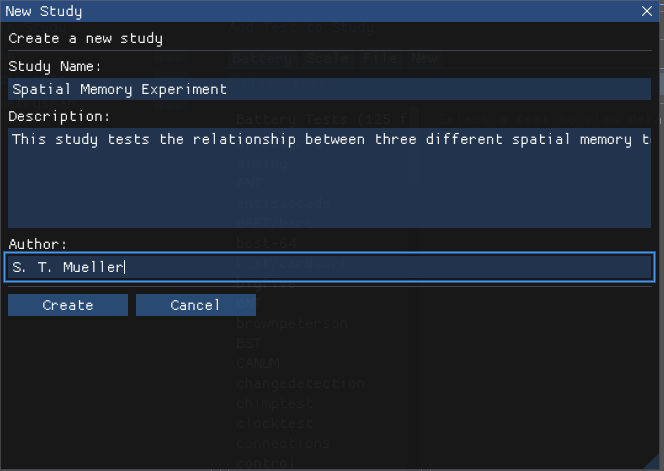
\includegraphics[width=0.55\textwidth]{images/launcher-new-study.png}
\end{figure}

\subsection{Tests sub-tab}

The Tests sub-tab lists all tests (PEBL battery tasks) and
scales/surveys available for use in this study.  You can browse the
battery by category, search by name, and view the description and
parameters of any test before adding it to a chain.

\begin{figure}[h]
\caption{The Tests sub-tab showing the battery task browser.}
\center
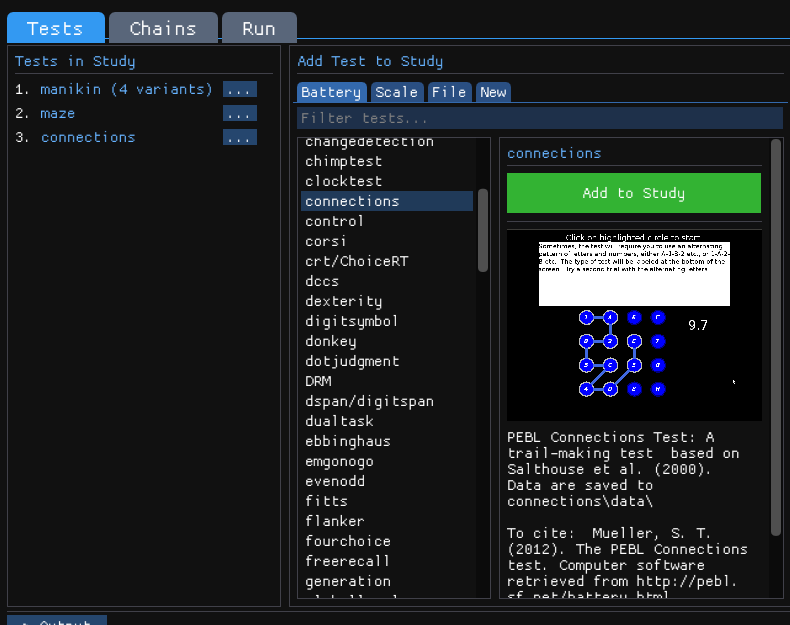
\includegraphics[width=0.85\textwidth]{images/launcher-tests-tab.png}
\end{figure}

\subsection{Chains sub-tab}
\label{sec:chains}

A chain is a sequence of items --- tests, scales, instruction pages,
consent forms, and completion screens --- run in order for each
participant.  Chains are the recommended way to deploy experiments,
even when running only a single test, because they manage participant
codes and data logging automatically.

\begin{figure}[h]
\caption{The Chains sub-tab showing a chain with several items.}
\center
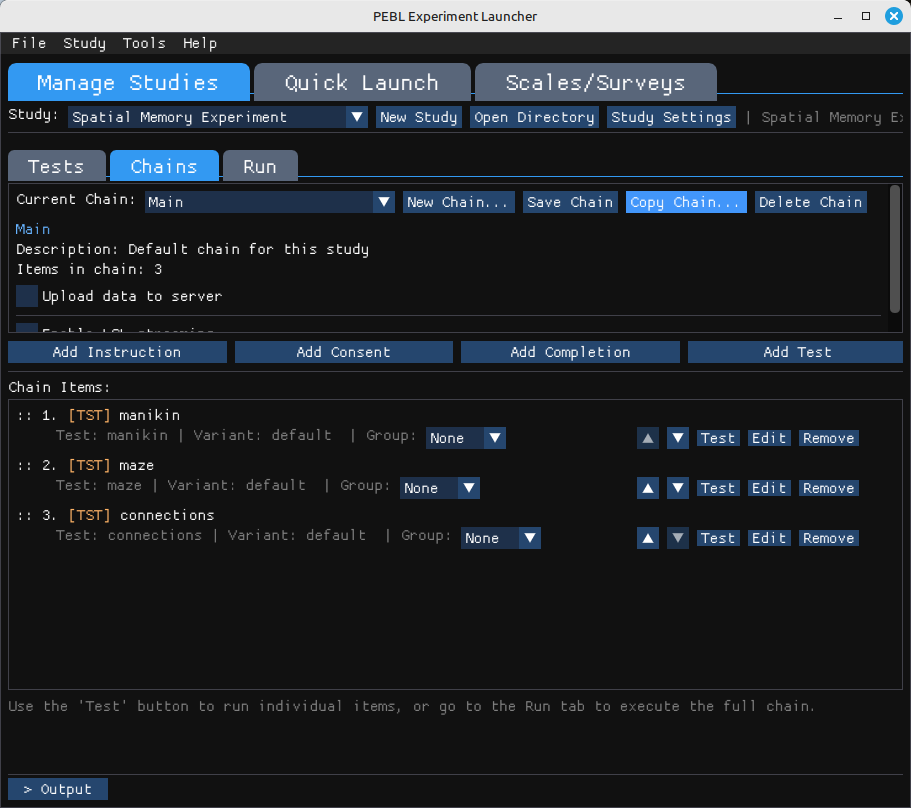
\includegraphics[width=0.85\textwidth]{images/launcher-chains-tab.png}
\end{figure}

\subsubsection{Creating and editing chains}

Use the \texttt{+} button to create a new chain, or select an existing
chain to edit it.  Each item in the chain can be:

\begin{itemize}
  \item \emph{Test} --- a battery task from \texttt{battery/}
  \item \emph{Scale/Survey} --- an OpenScales-format questionnaire
  \item \emph{Instruction} --- a text page shown to the participant
  \item \emph{Consent} --- a consent form; declining terminates the chain
  \item \emph{Completion} --- a final message shown at the end
\end{itemize}

Items can be reordered by dragging, and each item can have its own
parameter variant selected independently.

\begin{figure}[h]
\caption{Adding an item to a chain.  The item type selector and test browser are shown.}
\center
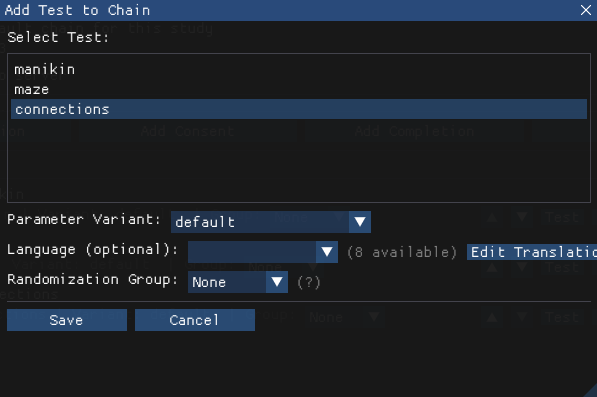
\includegraphics[width=0.75\textwidth]{images/launcher-chain-add-item.png}
\end{figure}

\subsubsection{Participant code}

The chain settings panel lets you configure the participant code
prefix, numeric counter, and session identifier.  The counter is
incremented automatically after each successful chain run.  You can
also edit it manually via the \emph{Edit Participant Code} dialog.

\begin{figure}[h]
\caption{The Edit Participant Code dialog.}
\center
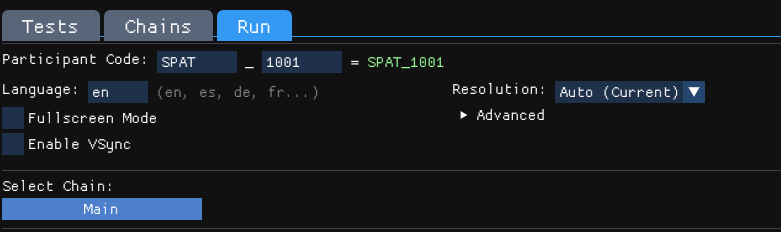
\includegraphics[width=0.5\textwidth]{images/launcher-participant-code.png}
\end{figure}

\subsubsection{Language}

Set the two-letter ISO 639-1 language code (e.g., \texttt{en},
\texttt{es}, \texttt{fr}) to control which translations are loaded by
experiments that support multiple languages.  If a translation for the
selected language is unavailable, experiments fall back to English.

\subsubsection{Fullscreen mode}

Check \emph{Fullscreen} to launch experiments without window
decorations.  To abort a running experiment at any time, press \verb|Ctrl+Alt+Shift+\|.

\subsubsection{Running a chain}

Click \emph{Run Chain} to execute all items in sequence.  The launcher
starts each item as a separate \texttt{pebl2} process and advances
automatically when each item finishes.  Output (stdout/stderr) from all
items in the chain is accumulated and displayed in the Run tab when the
chain completes.

\subsection{Run sub-tab}

The Run sub-tab shows the accumulated standard output and error output
from the most recently executed chain.  Separate panels display stdout
(from \texttt{Print()} calls) and stderr (status messages and error
diagnostics).  This is the first place to check if an experiment
crashes or produces unexpected output.

\begin{figure}[h]
\caption{The Run sub-tab showing stdout and stderr output after a chain completes.}
\center
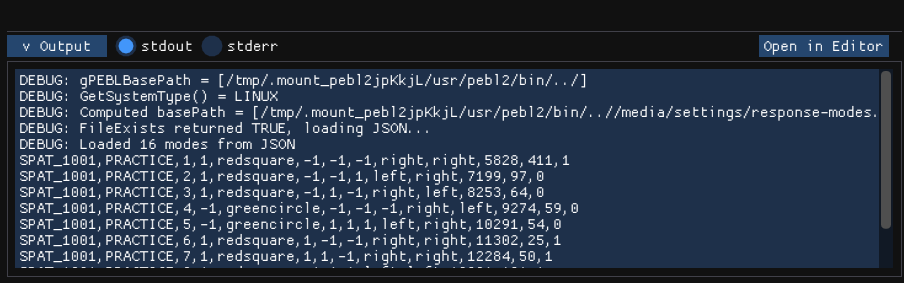
\includegraphics[width=0.85\textwidth]{images/launcher-run-tab.png}
\end{figure}


\sect{Quick Launch}

The Quick Launch tab provides a simple file browser for running any
\texttt{.pbl} file without setting up a study or chain.  This is
useful for testing scripts during development.

Navigate to the desired directory in the file browser; only
\texttt{.pbl} files and subdirectories are shown.  Select a file and
click \emph{Run} to execute it with the current participant code,
language, and fullscreen settings.

\begin{figure}[h]
\caption{The Quick Launch tab with a \texttt{.pbl} file selected.}
\center
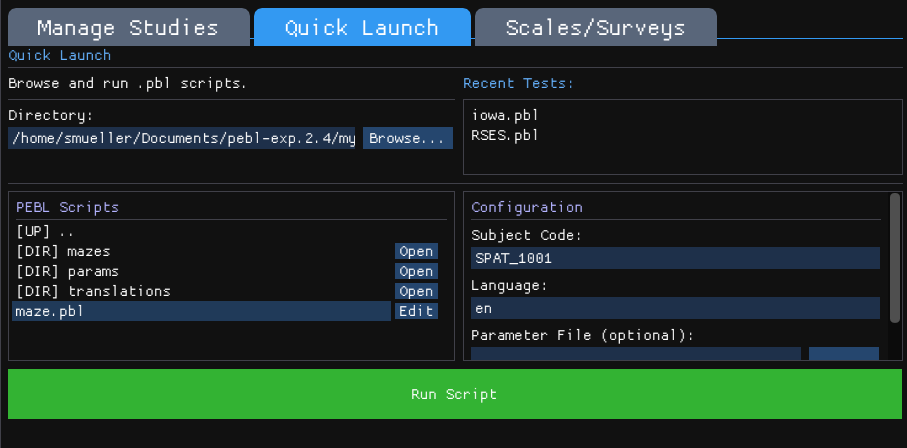
\includegraphics[width=0.85\textwidth]{images/launcher-quick-launch.png}
\end{figure}


\sect{Scales/Surveys (Scale Builder)}

The Scales/Surveys tab is a built-in editor for creating and editing
psychological scales and surveys in OpenScales Definition (OSD) format.
It provides sub-tabs for:

\begin{description}
\item[Scale Info] Name, description, author, version, and licensing
  metadata.
\item[Questions] Add, edit, and reorder individual items.  Supports
  multiple response formats: Likert, multiple choice, multicheck,
  text entry, and more.
\item[Dimensions \& Scoring] Define subscales and scoring rules.
\item[Translations] Manage translations of item text and response
  labels into multiple languages.
\item[Sections] Organize items into sections with optional headers.
\item[Parameters] Set default display parameters (number of response
  options, scale labels, randomization, etc.).
\end{description}

Scales created or edited here are stored as \texttt{.osd.json} files
in your study directory.  They can be run directly via the chain system
or shared with other researchers.

\begin{figure}[h]
\caption{The Scale Builder showing the Questions sub-tab with an item open for editing.}
\center
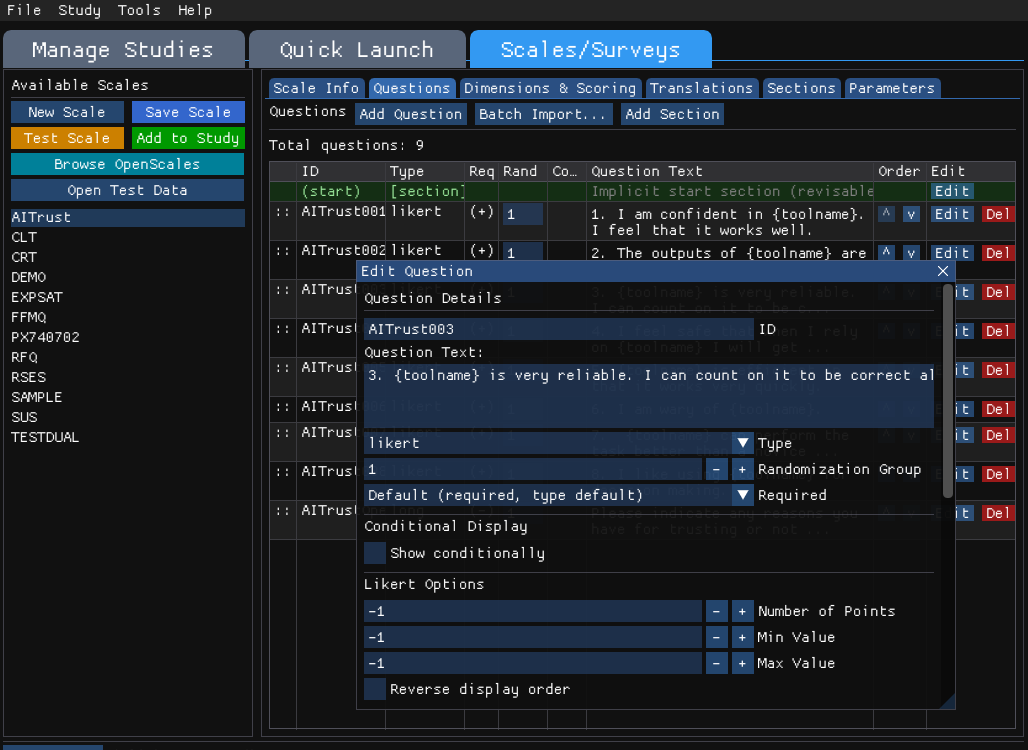
\includegraphics[width=0.85\textwidth]{images/launcher-scale-builder.png}
\end{figure}


\sect{Settings}

The Settings dialog (accessible from \emph{File \textbar{} Settings})
contains three panels:

\begin{description}
\item[General] Language code, fullscreen default, and font size.
\item[File Paths] Battery path (location of the \texttt{battery/}
  directory), PEBL executable path, and data output directory.
\item[Upload] Configuration for the PEBL data upload system
  (\texttt{--upload} option), including the server URL and
  authentication token.
\end{description}

Settings are saved to a configuration file in the workspace directory
and restored on next launch.

\begin{figure}[h]
\caption{The Settings dialog showing the File Paths panel.}
\center
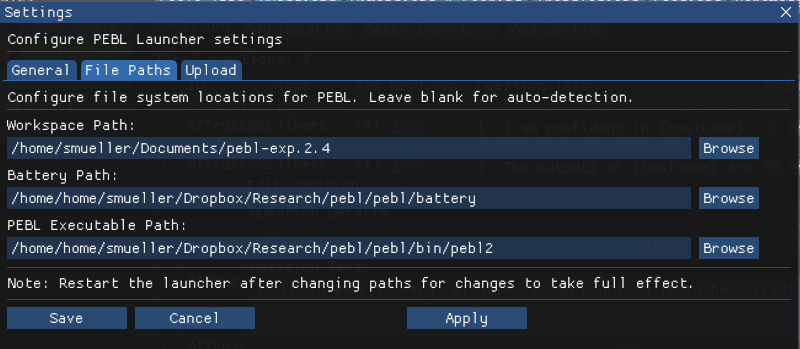
\includegraphics[width=0.6\textwidth]{images/launcher-settings.png}
\end{figure}


\sect{Snapshots}

Snapshots allow you to package a study (including its chains,
parameters, and scale definitions but excluding participant data) into
a portable archive that can be shared with colleagues or deployed to a
new machine.

\begin{itemize}
  \item \emph{Create Snapshot} --- archives the current study into the
    \texttt{snapshots/} folder in your workspace.
  \item \emph{Import Snapshot} --- unpacks a snapshot archive into
    \texttt{my\_studies/} as a new study ready to run.
\end{itemize}


\sect{Menu Reference}

\begin{description}
\item[File \textbar{} New Study] Create a new study in the workspace.
\item[File \textbar{} Open Study] Open an existing study directory.
\item[File \textbar{} Save] Save the current chain or scale.
\item[File \textbar{} Import Snapshot] Import a shared study snapshot.
\item[File \textbar{} Settings] Open the Settings dialog.
\item[File \textbar{} Exit] Close the launcher (saves configuration
  automatically).
\item[Help \textbar{} Manual] Open the PDF manual.  On installed mode, the
  manual is found in \texttt{Documents/pebl-exp.2.4/doc/}.  On portable
  mode, it is at the distribution root.
\item[Help \textbar{} Website] Open the PEBL website in a browser.
\item[Help \textbar{} About] Display version and license information.
\end{description}


\sect{Utility: Combining Data Files}

Once an experiment session is complete, participant data files are
stored within the \texttt{data/} subdirectory of the relevant battery
task.  When running via the launcher chain system, each participant's
files are organized by participant code.

To merge all data files into a single spreadsheet, use the PEBL data
combining utility, accessible from the Quick Launch tab or by running:
\begin{verbatim}
pebl2 /usr/local/share/pebl2/pebl-lib/combinedatafiles.pbl
\end{verbatim}

Navigate to the data directory of your test, then configure the match
and exclude patterns to select the files you want merged:

\begin{itemize}
  \item The match box filters by substring (e.g., \texttt{csv} selects
    only CSV files).  Separate multiple patterns with spaces (logical
    OR) or use \texttt{|}.  Use \texttt{\&} for AND (e.g.,
    \texttt{300\&csv} matches CSV files from participant 300).
  \item The exclude box removes matching files from the selection.
  \item Check \emph{Files contain header} to strip per-file headers and
    include a single header in the merged output.
  \item Check \emph{Add filename to data} to prepend a column
    identifying each row's source file.
  \item Use \emph{Combine and Save} to write the merged file, or
    \emph{Combine and Open} to also open it in the associated
    application.
\end{itemize}

%%% Local Variables:
%%% mode: latex
%%% TeX-master: "main"
%%% End:
